\section{Construction of Kerr Black-Hole Shadows}
\label{sec:shadow_construction}

\subsection{Celestial Bardeen Impact Parameters}
An asymptotic observer situated at Boyer--Lindquist radial distance $r_o \to \infty$ and polar inclination $\theta_o \in (0, \pi)$ views the black hole against a bright background. Photons that originate at infinity and are captured by the event horizon form a region of darkness on the observer's sky: the black hole shadow \cite{Bardeen1973,CunninghamBardeen1972,CunninghamBardeen1973,Falcke2000}.

The boundary of this shadow corresponds to the critical trajectories separating capture from scattering, which originate asymptotically from unstable spherical photon orbits (orbits of constant Boyer--Lindquist coordinate radius $r$) in the vicinity of the black hole.

Following Bardeen \cite{Bardeen1973}, we define celestial Cartesian screen coordinates $(\alpha, \beta)$ on the observer's sky, where $\alpha$ measures the horizontal impact parameter perpendicular to the projected black hole spin axis, and $\beta$ measures the vertical impact parameter parallel to the spin axis:
\begin{align}
    \alpha &\equiv -\frac{\xi}{\sin\theta_o}, \label{eq:bardeen_alpha} \\
    \beta &\equiv \pm \sqrt{\eta + a^2\cos^2\theta_o - \xi^2\cot^2\theta_o}, \label{eq:bardeen_beta}
\end{align}
where $\xi \equiv L_z/E$ and $\eta \equiv \mathcal{Q}/E^2$ are the normalized conserved impact parameters \eqref{eq:impact_parameters_xi_eta}.

\subsection{Analytical Parameterization via Spherical Photon Orbits}
Spherical photon orbits at coordinate radius $r$ satisfy the simultaneous algebraic conditions:
\begin{equation}
    R(r) = 0, \qquad \frac{dR}{dr} = 0,
    \label{eq:spherical_orbit_conditions}
\end{equation}
where $R(r)$ is the null radial potential \eqref{eq:radial_potential_R} with $\mu = 0$. Eliminating $E$ yields the unique analytical parameterization for the conserved impact parameters of spherical orbits \cite{Bardeen1973,Chandrasekhar1983,Teo2003,Teo2021}:
\begin{align}
    \xi(r) &= \frac{M(r^2 - a^2) - r\Delta(r)}{a(r - M)}, \label{eq:spherical_xi} \\
    \eta(r) &= \frac{r^3 \left[ 4Ma^2 - r(r - 3M)^2 \right]}{a^2(r - M)^2}. \label{eq:spherical_eta}
\end{align}

The physically accessible coordinate radius interval for exterior spherical photon orbits is bounded by the prograde and retrograde equatorial circular photon radii:
\begin{equation}
    r \in [r_{\rm ph}^+, r_{\rm ph}^-],
    \label{eq:spherical_radius_domain}
\end{equation}
where $r_{\rm ph}^\pm(a)$ are given by \eqref{eq:kerr_photon_orbit_radii}. On this interval, $\eta(r) \ge 0$, and the polar turning points of the orbits oscillate between $\theta_{\min}$ and $\pi - \theta_{\min}$ with:
\begin{equation}
    \cos^2\theta_{\min}(r) = \frac{\sqrt{(\eta + \xi^2 - a^2)^2 + 4a^2\eta} - (\eta + \xi^2 - a^2)}{2a^2}.
    \label{eq:spherical_theta_min}
\end{equation}

\subsection{Radial Offset Transformation and Root Isolation}
Direct numerical evaluation of \eqref{eq:bardeen_beta} for $r \approx 3M$ in floating-point arithmetic can suffer from catastrophic cancellation because $(r - 3M)^2$ subtracts two nearly equal quantities. To ensure scale-invariant precision down to machine epsilon, our implementation transforms to the offset radial variable:
\begin{equation}
    u \equiv r - 3M.
    \label{eq:offset_variable_u}
\end{equation}
In terms of $u$, the impact parameters become:
\begin{align}
    \xi(u) &= -\frac{u(9M^2 + 6Mu + u^2) + a^2(4M + u)}{a(2M + u)}, \label{eq:offset_xi} \\
    \eta(u) &= \frac{(3M + u)^3 \left(u - u_1\right)(u_{\rm max} - u)(u - u_{\rm min})}{a^2(2M + u)^2}, \label{eq:offset_eta}
\end{align}
where $u_{\rm min} = r_{\rm ph}^+ - 3M$, $u_{\rm max} = r_{\rm ph}^- - 3M$, and $u_1 = \frac{4Ma^2}{r_{\rm ph}^+ r_{\rm ph}^-} - 3M$.

The Carter vertical radicand function in \eqref{eq:bardeen_beta} is:
\begin{equation}
    B(u; \theta_o) \equiv \eta(u) + a^2\cos^2\theta_o - \xi(u)^2\cot^2\theta_o.
    \label{eq:carter_B_u}
\end{equation}
Real shadow boundary points require $B(u; \theta_o) \ge 0$. The roots $B(u; \theta_o) = 0$ define the admissible offset interval $[u_{\rm minus}, u_{\rm plus}] \subseteq [u_{\rm min}, u_{\rm max}]$, which is solved via Brent's method with bracketed tolerance $\Delta u < 10^{-15}M$.

\subsection{Smooth Cosine-Clustered Contour Construction}
\label{subsec:smooth_contour}
To construct a closed, smoothly sampled polygon free of clustering singularities near turning points, the upper shadow branch is parameterized by the angle $\phi \in [0, \pi]$:
\begin{equation}
    u(\phi) = \frac{u_{\rm plus} + u_{\rm minus}}{2} + \frac{u_{\rm plus} - u_{\rm minus}}{2} \cos\phi, \qquad \phi \in [0, \pi].
    \label{eq:cosine_clustered_u}
\end{equation}
At $\phi = 0$, $u = u_{\rm plus}$ ($r = r_{\max}$); at $\phi = \pi$, $u = u_{\rm minus}$ ($r = r_{\min}$). The vertical coordinate is evaluated as $\beta_{\rm upper}(\phi) = +\sqrt{B(u(\phi); \theta_o)}$, with $\beta(0) = \beta(\pi) \equiv 0$ enforced identically. The lower branch is obtained by reflecting across the equator: $\beta_{\rm lower}(\phi) = -\beta_{\rm upper}(\phi)$.

\subsection{Rendered Benchmark Shadows}
\Cref{fig:schwarzschild_shadow,fig:kerr_shadow_a05,fig:kerr_shadow_a09} illustrate the rendered scientific shadow boundaries for Schwarzschild ($a = 0$), intermediate Kerr ($a = 0.5M$), and rapidly rotating Kerr ($a = 0.9M$) at equatorial inclination $\theta_o = 90^\circ$:

\begin{figure}[!htbp]
    \centering
    \begin{minipage}[t]{0.48\textwidth}
        \centering
        \captionsetup{width=\linewidth}
        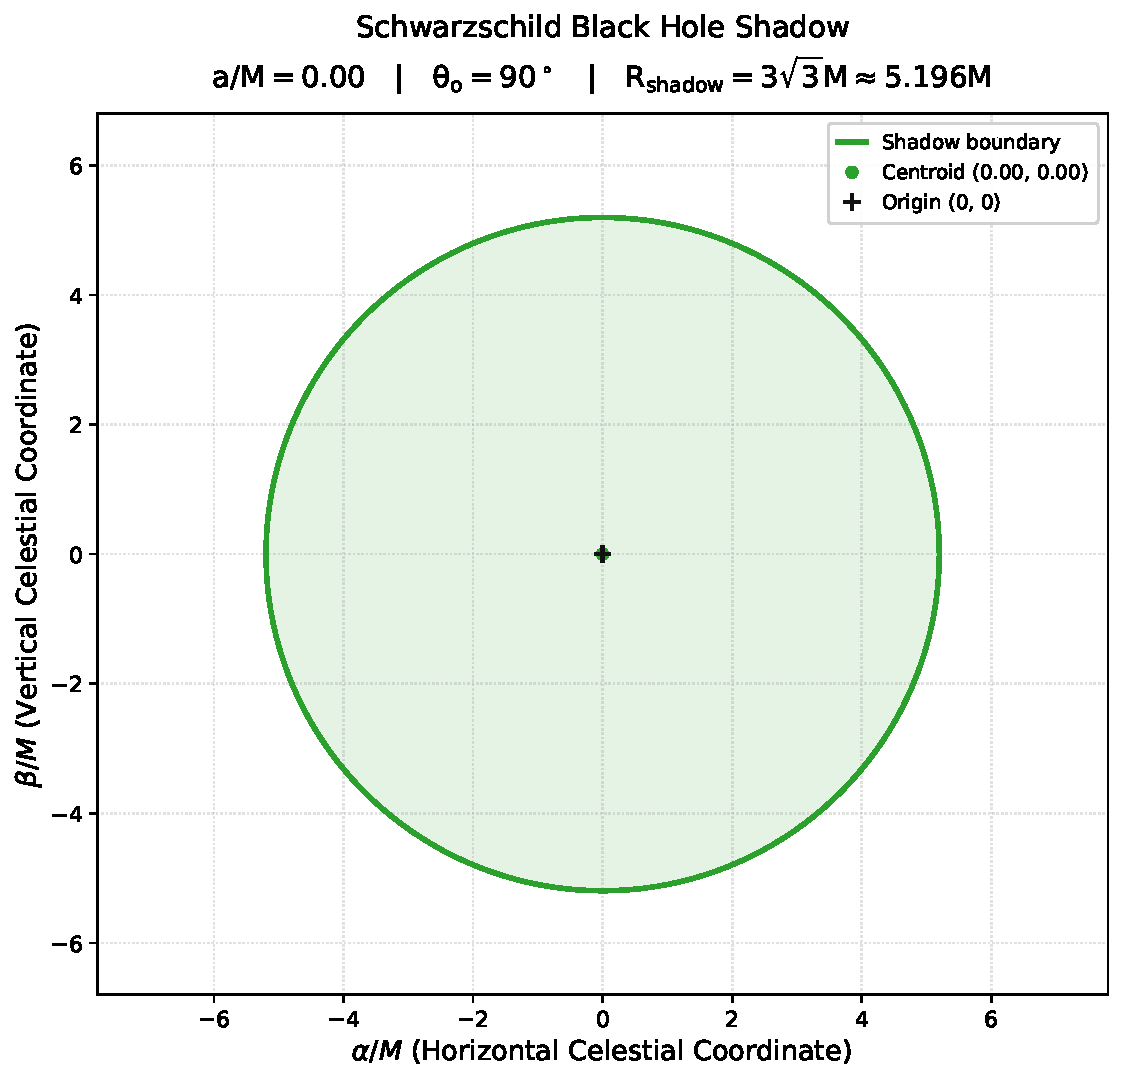
\includegraphics[width=\textwidth]{schwarzschild_shadow.pdf}
        \caption{The spherically symmetric Schwarzschild black hole shadow ($M = 1.0, a = 0$). The boundary is an exact circle centered at the origin with critical impact radius $R_{\rm circle} = 3\sqrt{3}M \approx 5.196M$ and enclosed area $A = 27\pi M^2 \approx 84.823M^2$.}
        \label{fig:schwarzschild_shadow}
    \end{minipage}
    \hfill
    \begin{minipage}[t]{0.48\textwidth}
        \centering
        \captionsetup{width=\linewidth}
        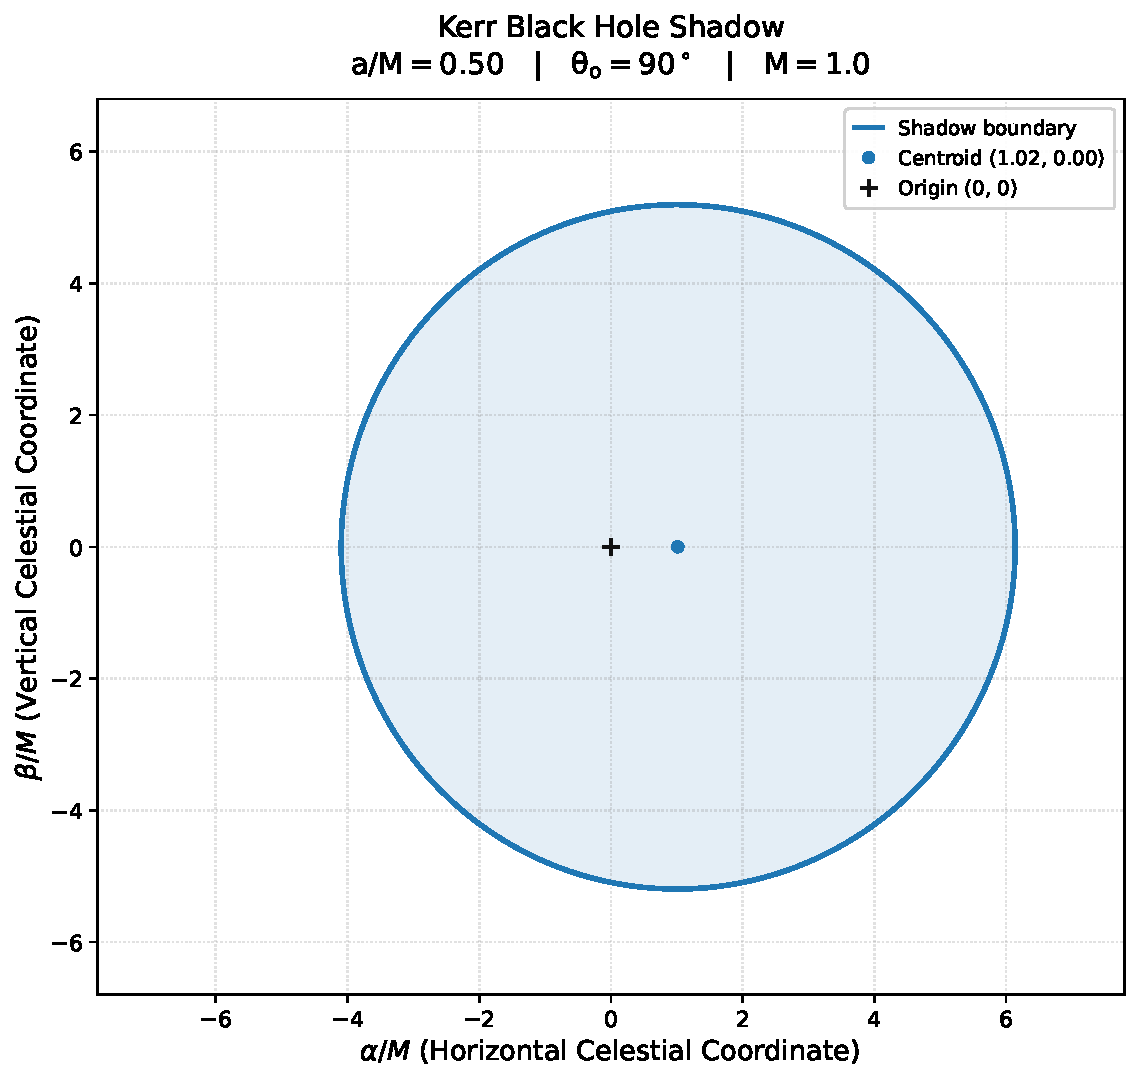
\includegraphics[width=\textwidth]{kerr_shadow_a05.pdf}
        \caption{Moderately rotating Kerr black hole shadow ($M = 1.0, a = 0.5M, \theta_o = 90^\circ$). Frame dragging shifts the retrograde boundary outwards and the prograde boundary inwards, displacing the horizontal centroid to $\bar{\alpha} = +1.02M$ while the vertical dimension remains symmetric ($A \approx 83.56M^2$).}
        \label{fig:kerr_shadow_a05}
    \end{minipage}
    \par\vspace{0.35cm}
    \begin{minipage}[t]{0.52\textwidth}
        \centering
        \captionsetup{width=\linewidth}
        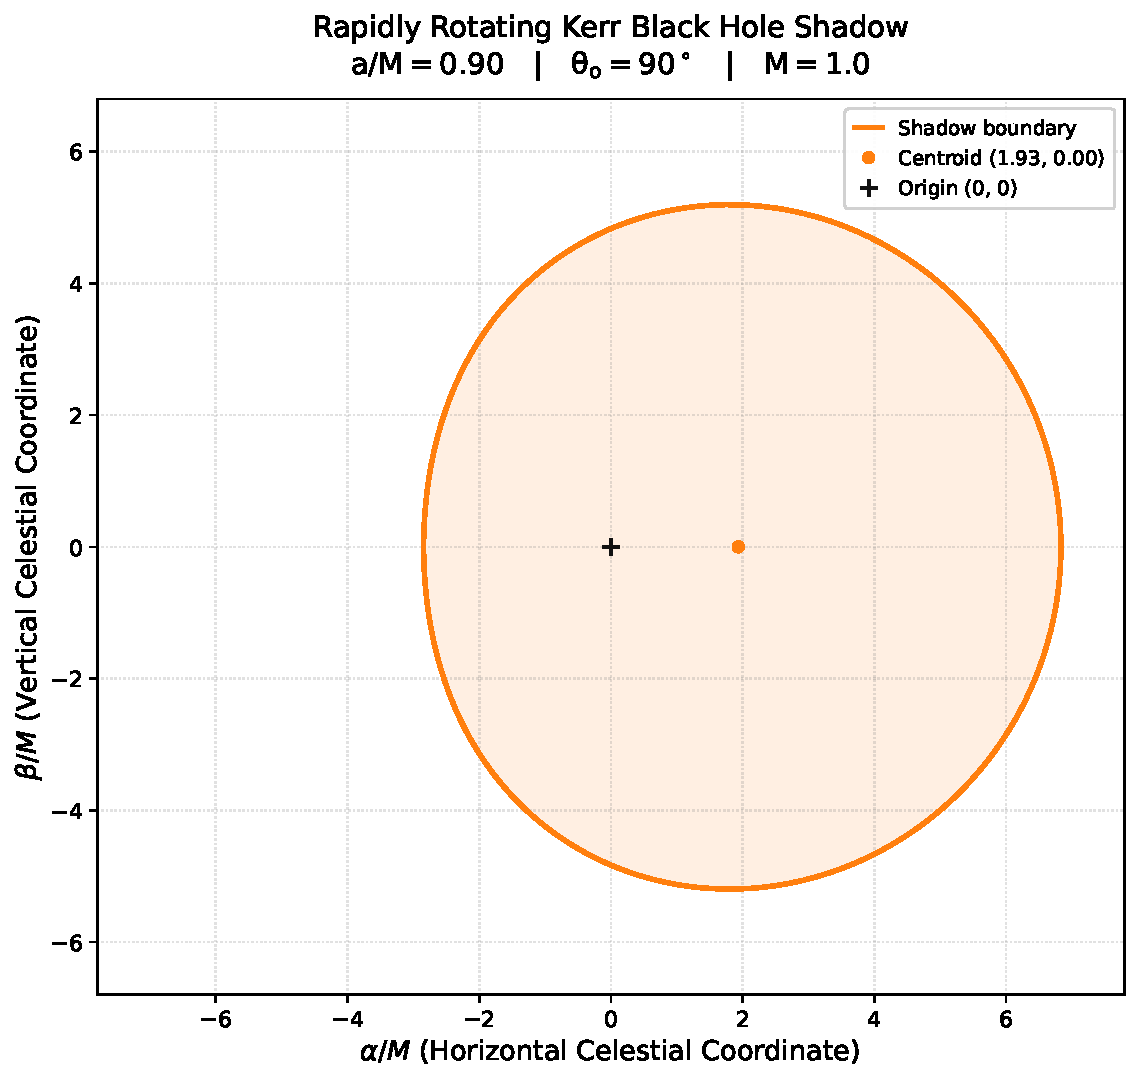
\includegraphics[width=\textwidth]{kerr_shadow_a09.pdf}
        \caption{Rapidly rotating Kerr black hole shadow ($M = 1.0, a = 0.9M, \theta_o = 90^\circ$). Strong frame-dragging shifts the prograde boundary to $\alpha_{\min} \approx -2.84M$ while the retrograde boundary extends to $\alpha_{\max} \approx +6.83M$, producing pronounced asymmetry ($A \approx 79.58M^2$, centroid $\bar{\alpha} = +1.93M$).}
        \label{fig:kerr_shadow_a09}
    \end{minipage}
\end{figure}

\subsection{Quantitative Shadow Observables Across Spin and Inclination}
\label{subsec:quantitative_shadow_observables}

To characterize the geometry of black-hole shadows quantitatively, we define five primary screen-plane observables for the closed boundary contour $\partial\Omega$ enclosing celestial region $\Omega$:
\begin{enumerate}[label=(\roman*)]
    \item \textbf{Celestial Shadow Area ($A/M^2$):}  
    The 2D planar Lebesgue measure of the shadow silhouette on the observer's screen:
    \begin{equation}
        A \equiv \iint_\Omega d\alpha\,d\beta = \frac{1}{2} \oint_{\partial\Omega} \left( \alpha\,d\beta - \beta\,d\alpha \right).
        \label{eq:area_def}
    \end{equation}
    For an open-array $N$-vertex polygon $(\alpha_i, \beta_i)_{i=0}^{N-1}$ with implicit cyclic closure $(\alpha_N, \beta_N) \equiv (\alpha_0, \beta_0)$, $A$ is evaluated via the discrete Shoelace formula:
    \begin{equation}
        A_N = \frac{1}{2} \left| \sum_{i=0}^{N-1} \left( \alpha_i \beta_{i+1} - \alpha_{i+1} \beta_i \right) \right|.
        \label{eq:shoelace_area}
    \end{equation}
    
    \item \textbf{Shadow Contour Perimeter ($P/M$):}  
    The total arc length of the closed boundary curve:
    \begin{equation}
        P \equiv \oint_{\partial\Omega} d\ell = \oint_{\partial\Omega} \sqrt{d\alpha^2 + d\beta^2}.
        \label{eq:perimeter_def}
    \end{equation}
    On the polygonal approximation, $P$ is computed by summing Euclidean chord lengths:
    \begin{equation}
        P_N = \sum_{i=0}^{N-1} \sqrt{ (\alpha_{i+1} - \alpha_i)^2 + (\beta_{i+1} - \beta_i)^2 }.
        \label{eq:polygonal_perimeter}
    \end{equation}

    \item \textbf{Horizontal Diameter ($D_{\mathrm{H}}/M$):}  
    The maximum projected extent of the shadow boundary curve parallel to the projected equatorial plane:
    \begin{equation}
        D_{\mathrm{H}} \equiv \alpha_{\max} - \alpha_{\min}.
        \label{eq:dh_def}
    \end{equation}

    \item \textbf{Vertical Diameter ($D_{\mathrm{V}}/M$):}  
    The maximum projected extent of the shadow boundary curve parallel to the projected spin axis:
    \begin{equation}
        D_{\mathrm{V}} \equiv \beta_{\max} - \beta_{\min}.
        \label{eq:dv_def}
    \end{equation}

    \item \textbf{Screen-Plane Area Centroid ($(\bar{\alpha}/M, \bar{\beta}/M)$):}  
    The center of mass of the enclosed planar domain $\Omega$:
    \begin{equation}
        \bar{\alpha} \equiv \frac{1}{A} \iint_\Omega \alpha\,d\alpha\,d\beta, \qquad
        \bar{\beta} \equiv \frac{1}{A} \iint_\Omega \beta\,d\alpha\,d\beta.
        \label{eq:centroid_def}
    \end{equation}
    Applying Green's theorem to the polygonal approximation yields the discrete moment formulas:
    \begin{align}
        \bar{\alpha}_N &= \frac{1}{6A_N} \sum_{i=0}^{N-1} (\alpha_i + \alpha_{i+1}) \left( \alpha_i \beta_{i+1} - \alpha_{i+1} \beta_i \right), \label{eq:centroid_alpha_poly} \\
        \bar{\beta}_N  &= \frac{1}{6A_N} \sum_{i=0}^{N-1} (\beta_i + \beta_{i+1}) \left( \alpha_i \beta_{i+1} - \alpha_{i+1} \beta_i \right). \label{eq:centroid_beta_poly}
    \end{align}
\end{enumerate}

\begin{table*}[t]
\centering
\small
\caption{Quantitative black hole shadow geometric observables across dimensionless spin $a/M$ and observer inclination $\theta_o$. All quantities are normalized by the black-hole mass: celestial area $A/M^2$, perimeter $P/M$, horizontal diameter $D_{\mathrm{H}}/M = \alpha_{\max} - \alpha_{\min}$, vertical diameter $D_{\mathrm{V}}/M = \beta_{\max} - \beta_{\min}$, and planar area centroid $(\bar{\alpha}/M, \bar{\beta}/M)$ computed via Green's theorem. Discrete polygonal values are evaluated at deliverable resolution $N=500$ (with $N=498$ for the piecewise-composite extremal contour). Reference values represent exact analytical limits where available (denoted with an asterisk $^*$), or independently computed high-resolution Richardson/quadrature benchmarks at $N=16\,384$. Equatorial reflection symmetry $\beta \leftrightarrow -\beta$ forces $\bar{\beta} = 0$ identically in the continuum; numerical values confirm $|\bar{\beta}_N| < 10^{-15}M$.}
\label{tab:shadow_observables}
\vspace{2mm}
\setlength{\tabcolsep}{4.5pt}
\begin{tabular}{lccccccccc}
\toprule
& & & \multicolumn{2}{c}{Area $A/M^2$} & \multicolumn{2}{c}{Perimeter $P/M$} & \multicolumn{2}{c}{Diameter $/M$} & Centroid \\
\cmidrule(lr){4-5} \cmidrule(lr){6-7} \cmidrule(lr){8-9}
Configuration & $a/M$ & $\theta_o$ & $N=500$ & Reference & $N=500$ & Reference & $D_{\mathrm{H}}$ & $D_{\mathrm{V}}$ & $\bar{\alpha}/M$ \\
\midrule
Schwarzschild & 0.00 & $90^\circ$ & 84.821 & 84.823$^*$ & 32.648 & 32.648$^*$ & 10.392 & 10.392 & 0.000 \\
Kerr & 0.50 & $90^\circ$ & 83.559 & 83.561 & 32.406 & 32.406 & 10.234 & 10.392 & 1.015 \\
Kerr & 0.90 & $90^\circ$ & 79.585 & 79.587 & 31.663 & 31.663 & 9.677 & 10.392 & 1.933 \\
Kerr & 0.90 & $45^\circ$ & 77.594 & 77.596 & 31.239 & 31.239 & 9.714 & 10.139 & 1.411 \\
Kerr & 0.90 & $15^\circ$ & 76.126 & 76.129 & 30.930 & 30.930 & 9.812 & 9.878 & 0.530 \\
Kerr (Polar) & 0.90 & $0^\circ$ & 75.923 & 75.925$^*$ & 30.888 & 30.889$^*$ & 9.832 & 9.832 & 0.000 \\
Extremal Kerr & 1.00 & $90^\circ$ & 76.243 & 76.246 & 31.177 & 31.177 & 9.000 & 10.392 & 2.288 \\
Extremal (Polar) & 1.00 & $0^\circ$ & 73.240 & 73.242$^*$ & 30.338 & 30.338$^*$ & 9.657 & 9.657 & 0.000 \\
\bottomrule
\end{tabular}
\end{table*}

\noindent \textbf{Important Methodological Distinction:} The area centroid $(\bar{\alpha}, \bar{\beta})$ must not be confused with the midpoint of the bounding box, $\left(\frac{\alpha_{\max} + \alpha_{\min}}{2}, \frac{\beta_{\max} + \beta_{\min}}{2}\right)$. Because black-hole frame dragging introduces severe left-right asymmetry, the bulk of the enclosed celestial area is weighted differently than the extremal points. For example, in rapidly rotating Kerr ($a = 0.9M, \theta_o = 90^\circ$), the bounding box midpoint lies at $\frac{6.832 - 2.844}{2} = 1.994M$, whereas the true area centroid is $\bar{\alpha} = 1.933M$, a significant physical discrepancy of $\Delta\alpha = 0.061M$.

\Cref{tab:shadow_observables} compiles the verified geometric observables across all eight standard configurations. Examination of these numerical results establishes four major relativistic trends:
\begin{enumerate}
    \item \textbf{Monotonic Area and Perimeter Contraction with Spin:}  
    At equatorial inclination ($\theta_o = 90^\circ$), increasing dimensionless spin $a/M$ from $0.00$ to $1.00$ monotonically reduces the enclosed celestial shadow area from $A = 84.823M^2$ to $76.246M^2$ (a net decrease of $10.1\%$). Similarly, the perimeter contracts monotonically from $P = 32.648M$ down to $31.177M$ (a $4.5\%$ decrease). This contraction reflects the increased binding energy and closer horizon approach permitted for prograde photon orbits.
    
    \item \textbf{Horizontal Compression and Invariance of Equatorial Vertical Diameter:}  
    As spin increases at $\theta_o = 90^\circ$, frame dragging selectively flattens the prograde boundary ($\alpha < 0$), compressing the horizontal diameter from $D_{\mathrm{H}} = 10.392M$ ($a=0$) to $D_{\mathrm{H}} = 9.677M$ ($a=0.9M$), reaching an exact integer value $D_{\mathrm{H}} = 9.000M$ in extremal Kerr ($a=1.0M$).  
    In stark contrast, the vertical diameter $D_{\mathrm{V}}$ remains rigorously invariant at:
    \begin{equation}
        D_{\mathrm{V}} = 6\sqrt{3}M \approx 10.392305M, \qquad (\theta_o = 90^\circ, \forall a \in [0, M]).
        \label{eq:dv_invariant}
    \end{equation}
    This remarkable invariance is established by distinguishing two geometric regimes. For rotating Kerr black holes ($0 < a \le M$), $\cot\theta_o = 0$ at equatorial inclination ($\theta_o = 90^\circ$), reducing \eqref{eq:bardeen_beta} to $\beta(r) = \pm\sqrt{\eta(r)}$ completely independent of $\xi(r)$. Vertical boundary extrema thus occur where $d\eta/dr = 0$. Decomposing \eqref{eq:spherical_eta} as:
    \begin{equation}
        \eta(r) = \frac{4Mr^3}{(r-M)^2} - \frac{r^4(r-3M)^2}{a^2(r-M)^2}, \qquad (0 < a \le M),
        \label{eq:eta_decomposition_kerr}
    \end{equation}
    demonstrates that both rational terms have identically vanishing radial derivatives at $r = 3M$, yielding $\eta(3M) = 27M^2$, $\eta'(3M) = 0$, and $\eta''(3M) < 0$. This establishes $\beta_{\max} = \sqrt{27}M = 3\sqrt{3}M$ and $D_{\mathrm{V}} = 2\beta_{\max} = 6\sqrt{3}M$, with horizontal coordinate $\alpha = -\xi(3M) = +2a$ displaced toward the retrograde screen hemisphere. In the non-rotating Schwarzschild limit ($a = 0$), where the $1/a^2$ factor is formally singular, spherical symmetry independently dictates that the shadow is an exact circle of radius $R_{\rm circle} = 3\sqrt{3}M \approx 5.196M$ (cf.~Section~\ref{subsec:schwarzschild_photon_sphere}), establishing identically $D_{\mathrm{V}} = 2 R_{\rm circle} = 6\sqrt{3}M$. As $a \to 0$, the horizontal displacement $\alpha = +2a$ continuously tends to zero, smoothly recovering the unshifted, symmetric Schwarzschild boundary vertices at $(\alpha, \beta) = (0, \pm 3\sqrt{3}M)$.

    \item \textbf{Retrograde Centroid Displacement:}  
    Because $\alpha = -\xi/\sin\theta_o$, prograde photon orbits ($\xi > 0$) map to the negative $\alpha$ hemisphere, whereas retrograde orbits ($\xi < 0$) map to the positive $\alpha$ hemisphere. Prograde orbits can orbit much closer to the horizon ($r_{\rm ph}^+ \to M$), requiring smaller impact parameters and compressing the prograde boundary to $\alpha_{\min} \ge -2M$. Retrograde orbits remain distant ($r_{\rm ph}^- \to 4M$), extending the retrograde boundary to $\alpha_{\max} = +7M$ in extremal Kerr. Consequently, frame dragging shifts the centroid systematically toward the positive (retrograde) screen coordinate, increasing from $\bar{\alpha} = 0.000M$ to $+1.015M$ ($a=0.5M$), $+1.933M$ ($a=0.9M$), and $+2.288M$ ($a=1.0M$).

    \item \textbf{Smooth Circular Restoration Across Observer Inclinations:}  
    For a rapidly rotating black hole ($a=0.9M$), decreasing observer inclination from edge-on ($\theta_o = 90^\circ$) to face-on ($\theta_o = 0^\circ$) systematically eliminates the projected frame-dragging distortion. The centroid displacement $\bar{\alpha}$ smoothly subsides from $+1.933M$ ($\theta_o=90^\circ$) to $+1.411M$ ($45^\circ$), $+0.530M$ ($15^\circ$), and vanishes identically at $\theta_o = 0^\circ$. Simultaneously, $D_{\mathrm{H}}$ and $D_{\mathrm{V}}$ converge from an aspect ratio of $D_{\mathrm{H}}/D_{\mathrm{V}} \approx 0.931$ to an exact circle with $D_{\mathrm{H}} = D_{\mathrm{V}} = 9.832M$.
\end{enumerate}
